\section{Results} \label{sec:results}
Here the results will be presented. We start looking at how good our linear regression is, by fitting a polynomial to points withdrawn from a known PDF. Thereafter we will see how good the regression is when using real terrain data. To give an intuition on how good the fit is, we will in both cases show 3D plots of the polynomials given by OLS, Ridge and Lasso methods, and then present a proper error analysis. 

\subsection{Franke function}
Below one can find the results when fitting the Franke function. All results in this section were obtained from the same data set, consisting of 1000 points, withdrawn from a uniform distribution ($x,y\in[0,1]$). Further, the polynomial degrees in x- and y-directions were set to $P_x=P_y=5$. For the methods that require minimization, we used gradient descent with the parameters $\lambda=1e-5$ (penalty), $\eta=1e-4$ (learning rate) and $\text{niter}=1e5$ (number of iterations) when nothing else is specified. To benchmark the results (mainly to verify the code), Scikit Learn was used. In the first place, the studies were done without noise, and then everything was repeated with adding a noise of $\mathcal{N}(0, \sigma^2=0.1)$.

\subsubsection{Visualization of graphes}
In figure \eqref{fig:franke_plots} the polynomial produced by regression on noisy data is compared with the polynomial produced by regression on smooth data. 

 
\newgeometry{left=2cm,right=2cm,top=1cm}
\begin{figure} [H]%
    \centering
    \subfloat[OLS without noise]{{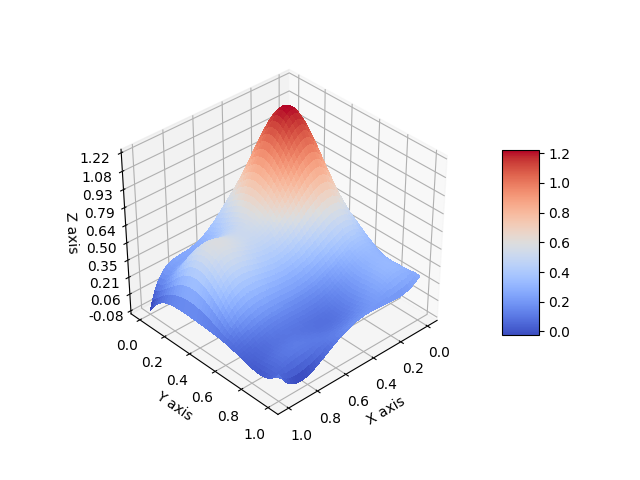
\includegraphics[width=9cm]{../plots/OLS.png} }}%
    \subfloat[OLS with noise]{{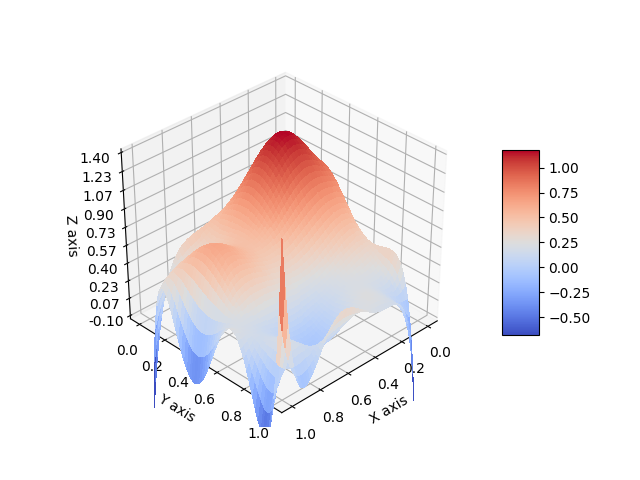
\includegraphics[width=9cm]{../plots/OLS_noise.png} }}\\

    \subfloat[Ridge without noise]{{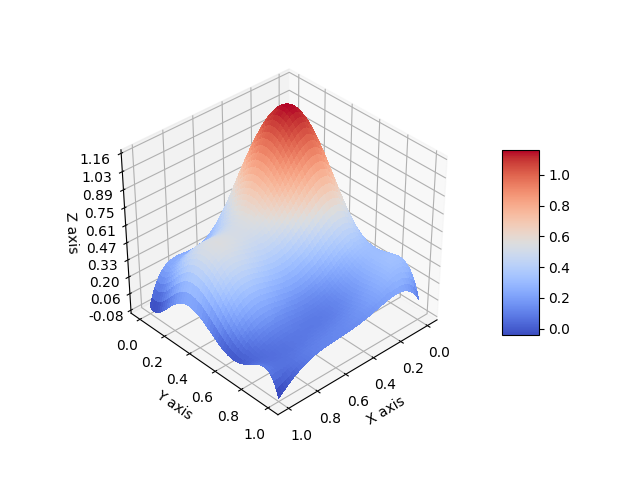
\includegraphics[width=9cm]{../plots/Ridge.png} }}%
    \subfloat[Ridge with noise]{{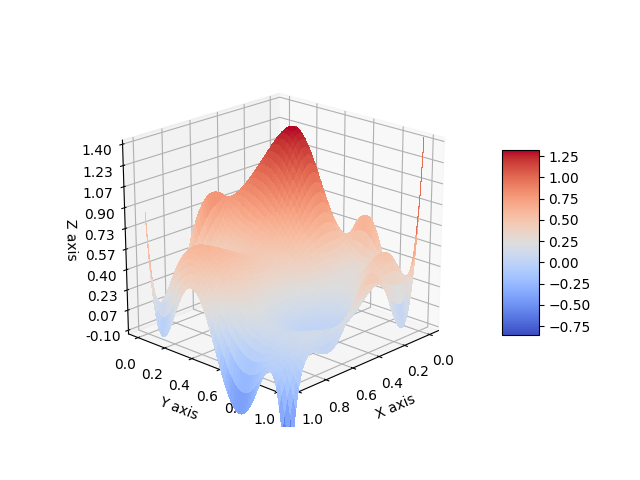
\includegraphics[width=9cm]{../plots/Ridge_noise.png} }}\\
    
    \subfloat[Lasso without noise]{{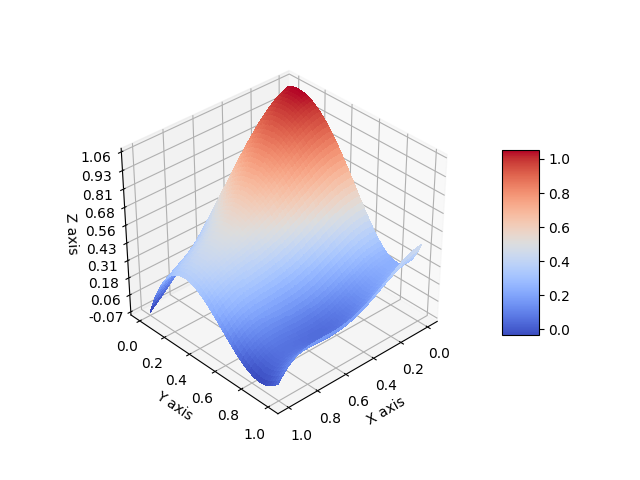
\includegraphics[width=9cm]{../plots/Lasso.png} }}%
    \subfloat[Lasso with noise]{{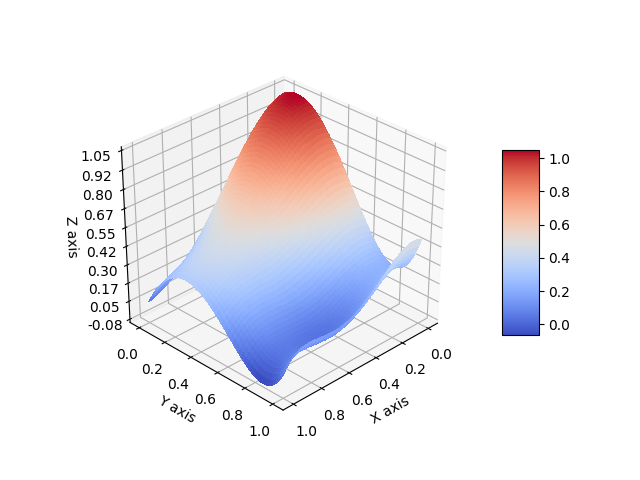
\includegraphics[width=9cm]{../plots/Lasso_noise.png} }}
    \caption{Fitted polynomial produced by OLS, Ridge and Lasso with (right hand side (RHS)) and without noise (left hand side (LHS)). For Ridge and Lasso, we used a low penalty of $\lambda=1e-5$. Lasso was performed with $\eta=1e-4$ and $\text{niter}=1e5$ iterations. The noise was sampled from a normal distribution with $\sigma^2=0.1$.}%
    \label{fig:franke_plots}%
\end{figure}
\restoregeometry


\subsubsection{Error}
To determine which method is best, we need to analyze the error. In table \eqref{tab:franke_error}, the MSE and R$^2$-score are given for OLS, Ridge, Lasso and Ridge with gradient descent (RidgeGD). The errors were evaluated by the self-implemented functions directly (Self), by K-fold resampling test data (K-fold) and by Scikit Learn (Scikit). 

\begin{table} [H]
	\caption{Mean Square Error and R$^2$-score presented for OLS, Ridge, Lasso and Ridge + gradient descent (RidgeGD), where noise was added to the data. The parameters used were $\lambda=1e-5$ (penalty), $\eta=1e-4$ (learning rate), $\text{niter}=1e5$ (number of iterations) and $\mathcal{N}(0, \sigma^2=0.1)$ (noise). See text for more information.}
	\begin{tabularx}{\textwidth}{l|XXX|XXX} \hline\hline
		\label{tab:franke_error}
		& \multicolumn{3}{c}{\textbf{MSE}}&\multicolumn{3}{c}{\textbf{R2}}\\ \hline
		&Self&K-fold&Scikit&Self&K-fold&Scikit\\ \hline \\
		OLS & 0.008494 & 0.009119 & 0.008494 & 0.9048 & 0.8956 & 0.9048 \\
		Ridge & 0.009128 & 0.009651 & 0.009128 & 0.8977 & 0.8895 & 0.8977 \\
		Lasso & 0.01439 & 0.01489 & 0.01555 & 0.8387 & 0.8296 & 0.8257 \\
		RidgeGD & 0.01451 & 0.01504 & 0.009128 & 0.8373 & 0.8280 & 0.8977 \\ \hline
	\end{tabularx}
\end{table}
We have also studied how the R$^2$ score is dependent on various parameters. In figure \eqref{fig:R2_scores}, the R$^2$-score is plotted as a function of the penalty for Ridge and Lasso (a), and as a function of the noise for OLS, Ridge and Lasso (b).

\begin{figure} [H]%
	\centering
	\subfloat[Lambda vs. R2-score]{{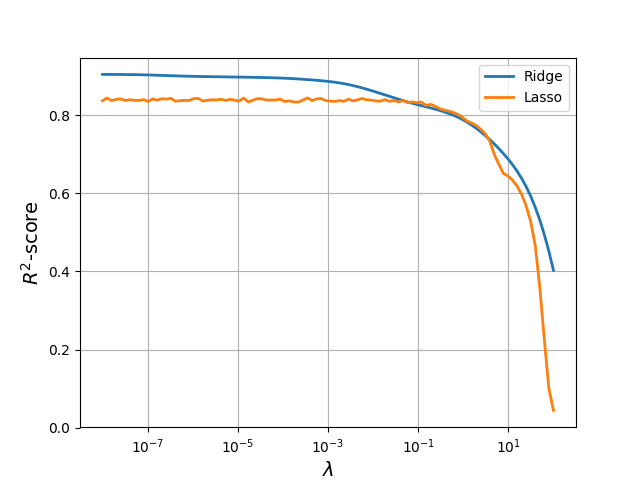
\includegraphics[width=7cm]{../plots/lambda_R2score.png} }}%
	\subfloat[Variance vs. R2-score]{{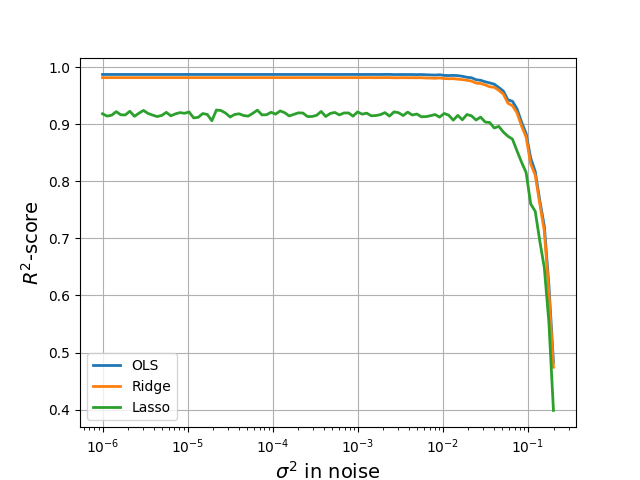
\includegraphics[width=7cm]{../plots/var_R2score.png} }}
	\caption{R$^2$-score plotted as a function of the penalty $\lambda$ (a) and as a function of the noise (b). $\lambda\in[10^{-8},10^2]$ in (a) and $\sigma^2\in[10^{-6},10^{-0.7}]$ in (b). The other parameters used were $\lambda=1e-5$ (penalty, was held constant for (b) only), $\eta=1e-4$ (learning rate), $niter=1e5$ (number of iterations) and $\mathcal{N}(0, \sigma^2=0.1)$ (noise, was held constant for (a) only).}%
	\label{fig:R2_scores}
\end{figure}

\subsubsection{Coefficients $\beta$}
It can also be interesting to see how the coefficients actually differ between the self-built functions and the Scikit Learn functions. In figure \eqref{fig:beta_plots}, the beta values are visualized such that large numbers got strong color, negative numbers are blue and positive numbers are red. The methods OLS, Ridge, Lasso and Ridge produced using gradient descent (RidgeGD) are presented. 

\begin{figure} [H]%
	\centering
	\subfloat[OLS self]{{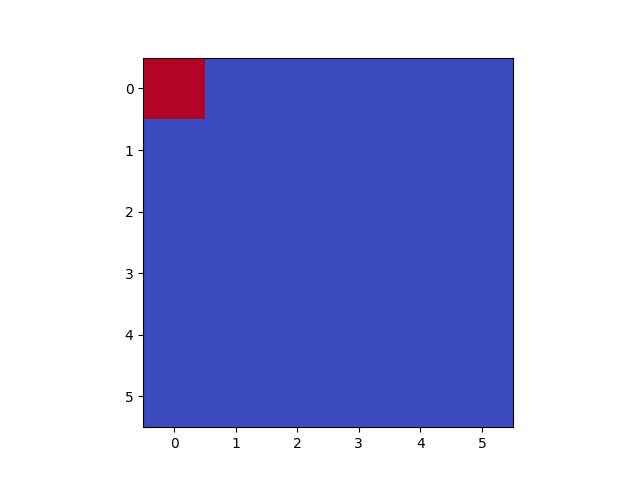
\includegraphics[width=3cm]{../plots/beta_ols_visualize.png} }}%
	\subfloat[Ridge self]{{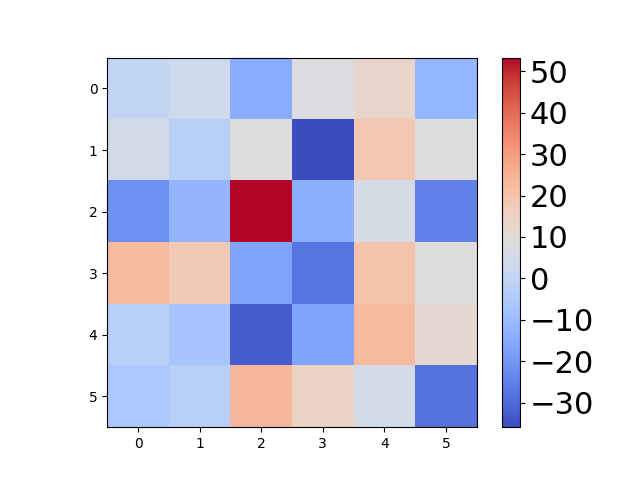
\includegraphics[width=3cm]{../plots/beta_ridge_visualize.png} }}%
	\subfloat[Lasso self]{{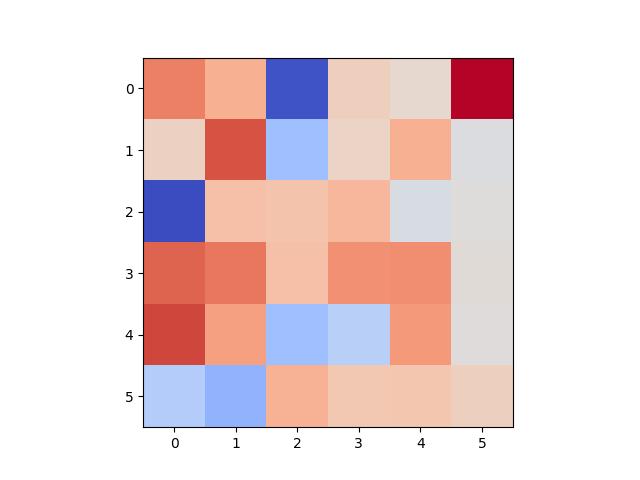
\includegraphics[width=3cm]{../plots/beta_lasso_visualize.png} }}%
	\subfloat[RidgeGD self]{{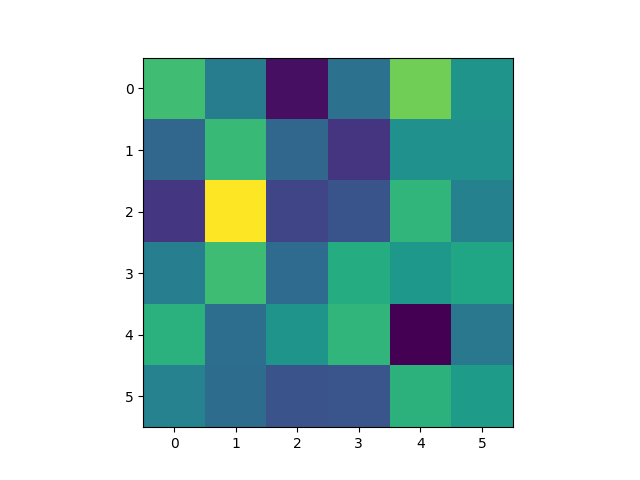
\includegraphics[width=3cm]{../plots/beta_ridge2_visualize.png} }}\\
	
	\subfloat[OLS scikit]{{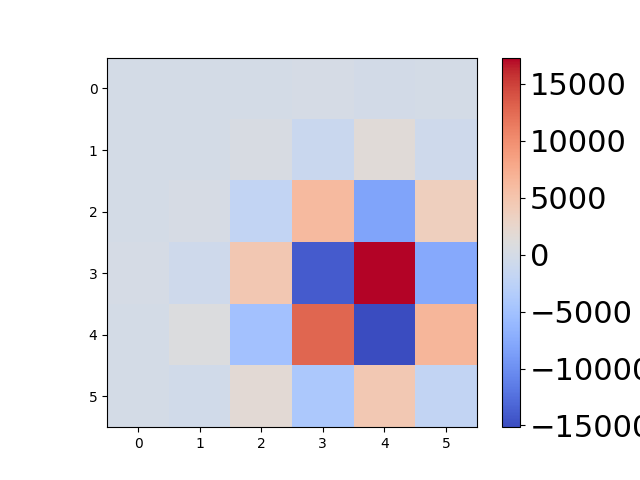
\includegraphics[width=3cm]{../plots/beta_ols_test_visualize.png} }}%
	\subfloat[Ridge scikit]{{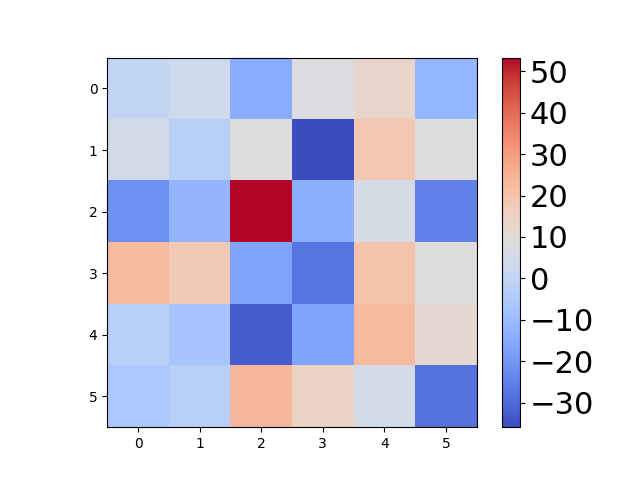
\includegraphics[width=3cm]{../plots/beta_ridge_test_visualize.png} }}%
	\subfloat[Lasso scikit]{{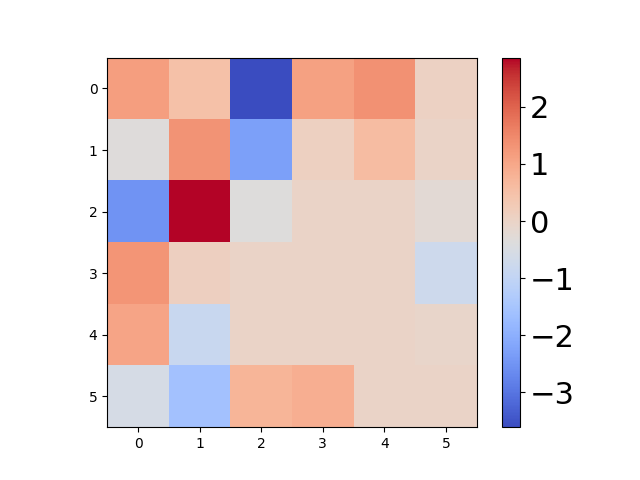
\includegraphics[width=3cm]{../plots/beta_lasso_test_visualize.png} }}%
	\subfloat[Ridge scikit]{{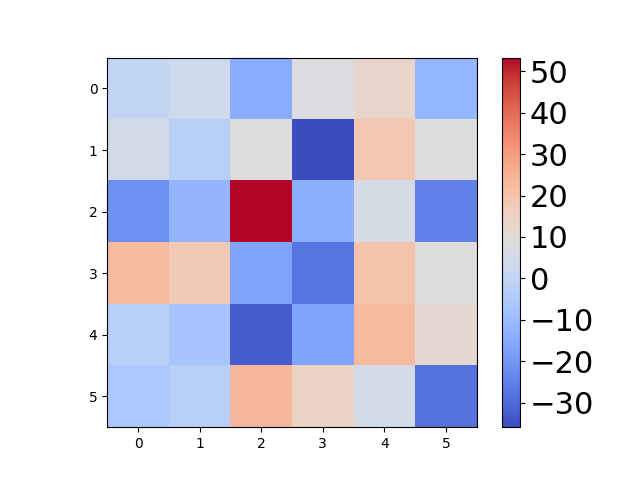
\includegraphics[width=3cm]{../plots/beta_ridge_test_visualize.png} }}
	
	\caption{Beta values visualized for various methods. The upper images were produced by the self-built functions, while the lower images are the benchmarks which were produced by Scikit learn. The parameters used were $\lambda=1e-5$ (penalty), $\eta=1e-4$ (learning rate), $\text{niter}=1e5$ (number of iterations) and $\mathcal{N}(0, \sigma^2=0.1)$ (noise).}%
	\label{fig:beta_plots}%
\end{figure}

\iffalse
Furthermore, the confidence intervals are given in table \eqref{tab:CI_franke} for all betas and all methods, when noise is included.

\begin{table} [H]
	\caption{Confidence intervals. The parameters used were $\lambda=1e-5$ (penalty), $\eta=1e-4$ (learning rate), $niter=1e5$ (number of iterations) and $\mathcal{N}(0, \sigma^2=0.01)$ (noise).  \vspace{2mm}}
	\begin{tabularx}{\textwidth}{l|XXXX} \hline\hline
		\label{tab:CI_franke}
		&\textbf{OLS}&\textbf{Ridge}&\textbf{Lasso}&\textbf{RidgeGD}\\ \hline \\
		$\beta_1$ & 0.07853 & 0.86104 & 0.05386 & 1.7483\\
		$\beta_2$ & 0.07853 & 0.86104 & 0.05386 & 1.7483\\
		$\beta_3$ & 0.07853 & 0.86104 & 0.05386 & 1.7483\\
		$\beta_4$ & 0.07853 & 0.86104 & 0.05386 & 1.7483\\
		$\beta_5$ & 0.07853 & 0.86104 & 0.05386 & 1.7483\\
		$\beta_6$ & 0.07853 & 0.86104 & 0.05386 & 1.7483\\
		$\beta_7$ & 0.07853 & 0.86104 & 0.05386 & 1.7483\\
		$\beta_8$ & 0.07853 & 0.86104 & 0.05386 & 1.7483\\
		$\beta_9$ & 0.07853 & 0.86104 & 0.05386 & 1.7483\\
		$\beta_{10}$ & 0.07853 & 0.86104 & 0.05386 & 1.7483\\
		$\beta_{11}$ & 0.07853 & 0.86104 & 0.05386 & 1.7483\\
		$\beta_{12}$ & 0.07853 & 0.86104 & 0.05386 & 1.7483\\
		$\beta_{13}$ & 0.07853 & 0.86104 & 0.05386 & 1.7483\\
		$\beta_{14}$ & 0.07853 & 0.86104 & 0.05386 & 1.7483\\
		$\beta_{15}$ & 0.07853 & 0.86104 & 0.05386 & 1.7483\\
		$\beta_{16}$ & 0.07853 & 0.86104 & 0.05386 & 1.7483\\
		$\beta_{17}$ & 0.07853 & 0.86104 & 0.05386 & 1.7483\\
		$\beta_{18}$ & 0.07853 & 0.86104 & 0.05386 & 1.7483\\
		$\beta_{19}$ & 0.07853 & 0.86104 & 0.05386 & 1.7483\\
		$\beta_{20}$ & 0.07853 & 0.86104 & 0.05386 & 1.7483\\
		$\beta_{21}$ & 0.07853 & 0.86104 & 0.05386 & 1.7483\\
		$\beta_{22}$ & 0.07853 & 0.86104 & 0.05386 & 1.7483\\
		$\beta_{23}$ & 0.07853 & 0.86104 & 0.05386 & 1.7483\\
		$\beta_{24}$ & 0.07853 & 0.86104 & 0.05386 & 1.7483\\
		$\beta_{25}$ & 0.07853 & 0.86104 & 0.05386 & 1.7483\\
		$\beta_{26}$ & 0.07853 & 0.86104 & 0.05386 & 1.7483\\
		$\beta_{27}$ & 0.07853 & 0.86104 & 0.05386 & 1.7483\\
		$\beta_{28}$ & 0.07853 & 0.86104 & 0.05386 & 1.7483\\
		$\beta_{29}$ & 0.07853 & 0.86104 & 0.05386 & 1.7483\\
		$\beta_{30}$ & 0.07853 & 0.86104 & 0.05386 & 1.7483\\
		$\beta_{31}$ & 0.07853 & 0.86104 & 0.05386 & 1.7483\\
		$\beta_{32}$ & 0.07853 & 0.86104 & 0.05386 & 1.7483\\
		$\beta_{33}$ & 0.07853 & 0.86104 & 0.05386 & 1.7483\\
		$\beta_{34}$ & 0.07853 & 0.86104 & 0.05386 & 1.7483\\
		$\beta_{35}$ & 0.07853 & 0.86104 & 0.05386 & 1.7483\\
		$\beta_{36}$ & 0.07853 & 0.86104 & 0.05386 & 1.7483\\ \hline
	\end{tabularx}
\end{table}
\fi

\subsection{Real data}
Below one can find the results when fitting the terrain data with a polynomial of a maximum degree of 5 in x- and y-directions. For the methods that require minimization, we used gradient descent with the parameters $\lambda=1e-5$ (penalty), $\eta=1e-4$ (learning rate) and $niter=1e5$ (number of iterations) when nothing else is specified. For benchmarking the results (mainly to verify the code), Scikit learn was used. In the first place, the studies were done without noise, and then everything was repeated with adding a noise of $\mathcal{N}(0, \sigma^2=0.1)$

\subsubsection{Visualization of graphes}
In figure \eqref{fig:terrain_plots}, we can see how good we were able to fit the polynomials using various methods


\newgeometry{left=2cm,right=2cm,top=1cm}
\begin{figure} [H]%
	\centering
	\subfloat[OLS]{{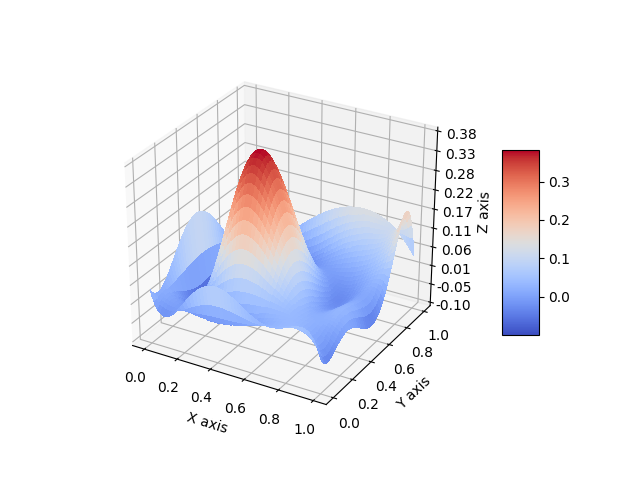
\includegraphics[width=9cm]{../plots/OLS_terrain.png} }}%
	\subfloat[Ridge]{{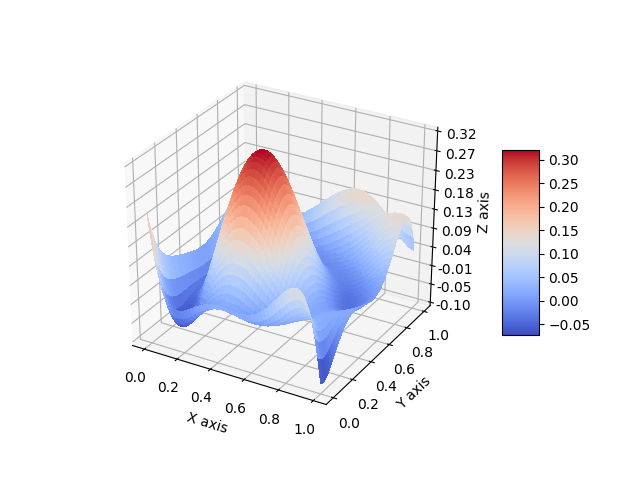
\includegraphics[width=9cm]{../plots/Ridge_terrain.png} }}\\
	
	\subfloat[Lasso]{{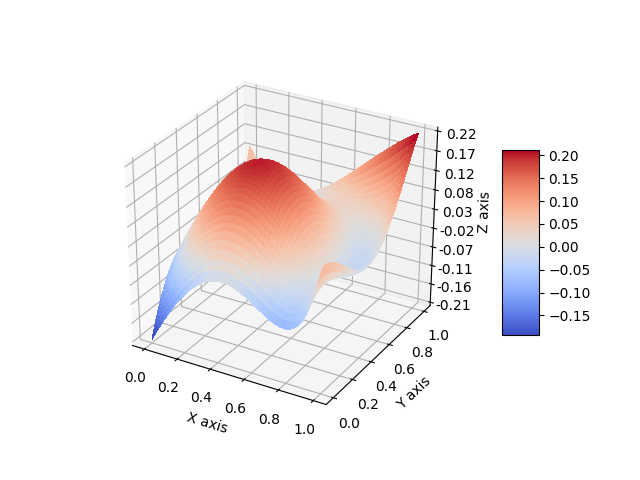
\includegraphics[width=9cm]{../plots/Lasso_terrain.png} }}%
	\subfloat[Terrain data]{{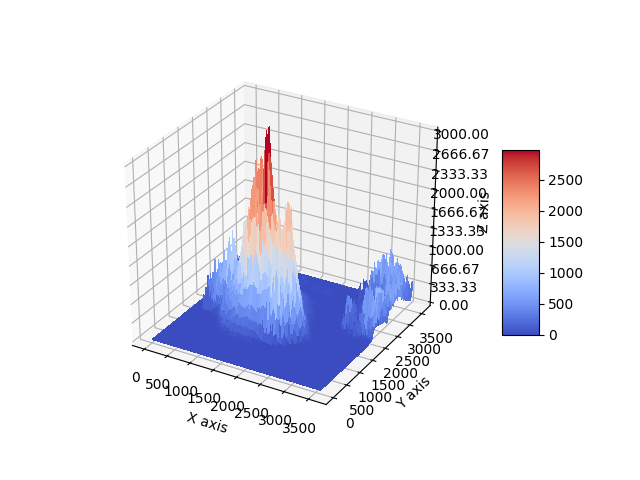
\includegraphics[width=9cm]{../plots/lombok.png} }}
	
	\caption{Fitted polynomial by OLS, Ridge and Lasso. For Ridge and Lasso, we used a low penalty of $\lambda=1e-5$. Lasso was performed with $\eta=1e-4$ and 1e5 iterations. The terrain data used in regression was normalized, but the data used in the terrain plot was not.}%
	\label{fig:terrain_plots}%
\end{figure}
\begin{figure} [H]
	\centering
	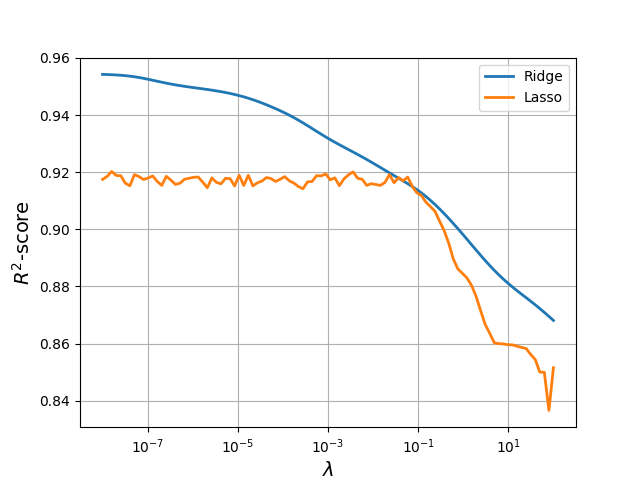
\includegraphics[width=7cm]{../plots/lambda_R2score_terrain.png}
	\caption{R$^2$-score plotted as a function of the penalty $\lambda$. The penalty was varied in the interval $\lambda\in[10^{-8},10^2]$, and the other parameters used were $\eta=1e-4$ (learning rate) and $niter=1e5$ (number of iterations).}
	\label{fig:R2_scores_terrain}
\end{figure}
\restoregeometry


\subsubsection{Error}
To be able to determine which method is best, we need to analyze the error. In table \eqref{tab:terrain_error}, the MSE and R$^2$-score are given for OLS, Ridge, Lasso and Ridge with gradient descent (RidgeGD). 

\begin{table} [H]
	\caption{Mean Square Error and R$^2$-score presented for OLS, Ridge, Lasso and Ridge + gradient descent (RidgeGD), where noise was added to the data. The parameters used were $\lambda=1e-5$ (penalty), $\eta=1e-4$ (learning rate), $niter=1e5$ (number of iterations) and $\mathcal{N}(0, \sigma^2=0.1)$ (noise). \vspace{2mm}}
	\begin{tabularx}{\textwidth}{l|XXX|XXX} \hline\hline
		\label{tab:terrain_error}
		& \multicolumn{3}{c}{\textbf{MSE}}&\multicolumn{3}{c}{\textbf{R2}}\\ \hline
		&self&K-fold&scikit&self&K-fold&scikit\\ \hline \\
		OLS & 0.006282 && 0.006282 & 0.9267 && 0.9267\\
		Ridge & 0.007886 && 0.007886 & 0.9080 && 0.9080 \\
		Lasso & 0.01294 && 0.01340 & 0.8491 && 0.8437 \\
		RidgeGD & 0.01299 && 0.007885 & 0.8485 && 0.9080 \\ \hline
	\end{tabularx}
\end{table}

We have also studied how the R$^2$ score is dependent on various parameters. In figure \eqref{fig:R2_scores_terrain}, the R$^2$-score is plotted as a function of the penalty for Ridge and Lasso (a), and as a function of the noise for OLS, Ridge and Lasso (b).


\iffalse
\subsubsection{Coefficients $\beta$}
It can also be interesting to see how the coefficients actually differ between the self-built functions and the Scikit Learn function. In figure \eqref{fig:beta_plots}, the beta values are visualized such that large numbers got strong color, negative numbers are blue and positive numbers are red. The methods OLS, Ridge, Lasso and Ridge produced using gradient descent (RidgeGD) are presented. 

Furthermore, the confidence intervals are given in table \eqref{tab:CI_terrain} for all betas and all methods, when noise is included.

\begin{table} [H]
	\caption{Confidence intervals. The parameters used were $\lambda=1e-5$ (penalty), $\eta=1e-4$ (learning rate), $niter=1e5$ (number of iterations) and $\mathcal{N}(0, \sigma^2=0.1)$ (noise).  \vspace{2mm}}
	\begin{tabularx}{\textwidth}{l|XXXX} \hline\hline
		\label{tab:CI_terrain}
		&\textbf{OLS}&\textbf{Ridge}&\textbf{Lasso}&\textbf{RidgeGD}\\ \hline \\
		$\beta_1$ & 0.07853 & 0.86104 & 0.05386 & 1.7483\\
		$\beta_2$ & 0.07853 & 0.86104 & 0.05386 & 1.7483\\
		$\beta_3$ & 0.07853 & 0.86104 & 0.05386 & 1.7483\\
		$\beta_4$ & 0.07853 & 0.86104 & 0.05386 & 1.7483\\
		$\beta_5$ & 0.07853 & 0.86104 & 0.05386 & 1.7483\\
		$\beta_6$ & 0.07853 & 0.86104 & 0.05386 & 1.7483\\
		$\beta_7$ & 0.07853 & 0.86104 & 0.05386 & 1.7483\\
		$\beta_8$ & 0.07853 & 0.86104 & 0.05386 & 1.7483\\
		$\beta_9$ & 0.07853 & 0.86104 & 0.05386 & 1.7483\\
		$\beta_{10}$ & 0.07853 & 0.86104 & 0.05386 & 1.7483\\
		$\beta_{11}$ & 0.07853 & 0.86104 & 0.05386 & 1.7483\\
		$\beta_{12}$ & 0.07853 & 0.86104 & 0.05386 & 1.7483\\
		$\beta_{13}$ & 0.07853 & 0.86104 & 0.05386 & 1.7483\\
		$\beta_{14}$ & 0.07853 & 0.86104 & 0.05386 & 1.7483\\
		$\beta_{15}$ & 0.07853 & 0.86104 & 0.05386 & 1.7483\\
		$\beta_{16}$ & 0.07853 & 0.86104 & 0.05386 & 1.7483\\
		$\beta_{17}$ & 0.07853 & 0.86104 & 0.05386 & 1.7483\\
		$\beta_{18}$ & 0.07853 & 0.86104 & 0.05386 & 1.7483\\
		$\beta_{19}$ & 0.07853 & 0.86104 & 0.05386 & 1.7483\\
		$\beta_{20}$ & 0.07853 & 0.86104 & 0.05386 & 1.7483\\
		$\beta_{21}$ & 0.07853 & 0.86104 & 0.05386 & 1.7483\\
		$\beta_{22}$ & 0.07853 & 0.86104 & 0.05386 & 1.7483\\
		$\beta_{23}$ & 0.07853 & 0.86104 & 0.05386 & 1.7483\\
		$\beta_{24}$ & 0.07853 & 0.86104 & 0.05386 & 1.7483\\
		$\beta_{25}$ & 0.07853 & 0.86104 & 0.05386 & 1.7483\\
		$\beta_{26}$ & 0.07853 & 0.86104 & 0.05386 & 1.7483\\
		$\beta_{27}$ & 0.07853 & 0.86104 & 0.05386 & 1.7483\\
		$\beta_{28}$ & 0.07853 & 0.86104 & 0.05386 & 1.7483\\
		$\beta_{29}$ & 0.07853 & 0.86104 & 0.05386 & 1.7483\\
		$\beta_{30}$ & 0.07853 & 0.86104 & 0.05386 & 1.7483\\
		$\beta_{31}$ & 0.07853 & 0.86104 & 0.05386 & 1.7483\\
		$\beta_{32}$ & 0.07853 & 0.86104 & 0.05386 & 1.7483\\
		$\beta_{33}$ & 0.07853 & 0.86104 & 0.05386 & 1.7483\\
		$\beta_{34}$ & 0.07853 & 0.86104 & 0.05386 & 1.7483\\
		$\beta_{35}$ & 0.07853 & 0.86104 & 0.05386 & 1.7483\\
		$\beta_{36}$ & 0.07853 & 0.86104 & 0.05386 & 1.7483\\ \hline
	\end{tabularx}
\end{table}
\fi